\begin{figuraNativa}[htbp]{Flujo operacional y cadena de valor del transporte de carga en Curimón}{2-flujo-operacional}
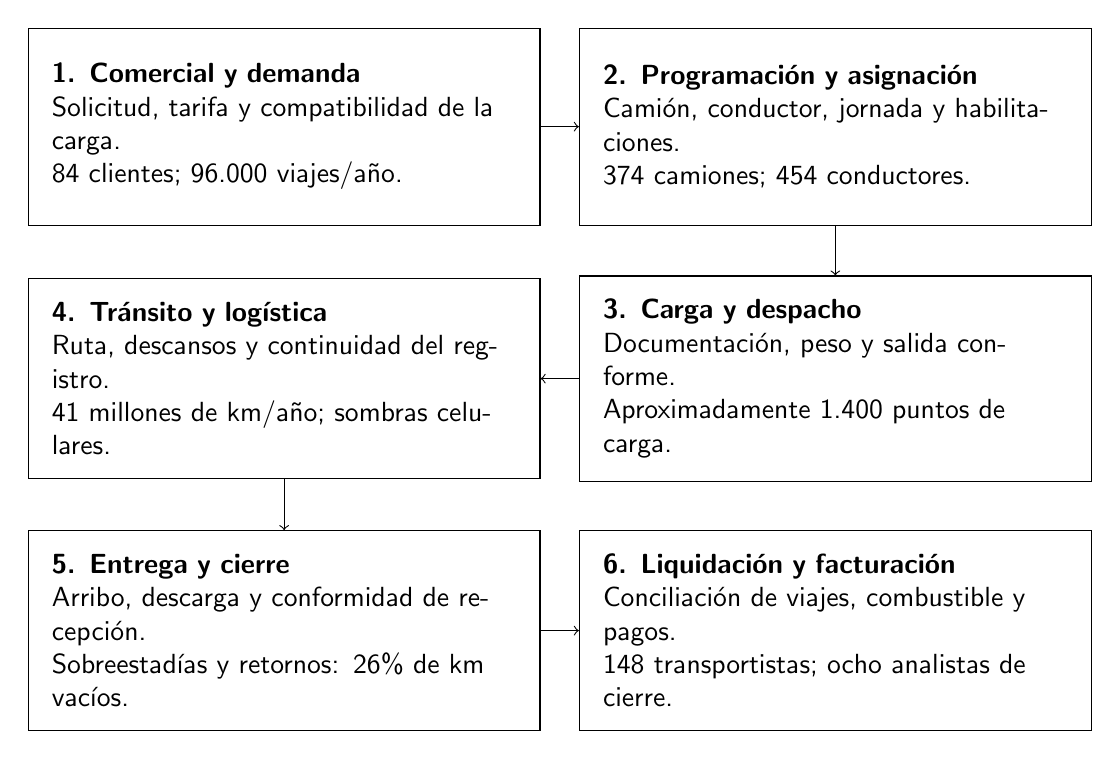
\begin{tikzpicture}[every node/.style={draw,align=left,text width=59mm,inner sep=3mm,minimum height=25mm,font=\sffamily\fontsize{9.5bp}{12bp}\selectfont}]
\node (a) at (0,0) {\textbf{1. Comercial y demanda}\\Solicitud, tarifa y compatibilidad de la carga.\\84 clientes; 96.000 viajes/año.};
\node (b) at (7,0) {\textbf{2. Programación y asignación}\\Camión, conductor, jornada y habilitaciones.\\374 camiones; 454 conductores.};
\node (c) at (7,-3.2) {\textbf{3. Carga y despacho}\\Documentación, peso y salida conforme.\\Aproximadamente 1.400 puntos de carga.};
\node (d) at (0,-3.2) {\textbf{4. Tránsito y logística}\\Ruta, descansos y continuidad del registro.\\41 millones de km/año; sombras celulares.};
\node (e) at (0,-6.4) {\textbf{5. Entrega y cierre}\\Arribo, descarga y conformidad de recepción.\\Sobreestadías y retornos: 26\% de km vacíos.};
\node (f) at (7,-6.4) {\textbf{6. Liquidación y facturación}\\Conciliación de viajes, combustible y pagos.\\148 transportistas; ocho analistas de cierre.};
\draw[->] (a.east)--(b.west);\draw[->] (b.south)--(c.north);\draw[->] (c.west)--(d.east);\draw[->] (d.south)--(e.north);\draw[->] (e.east)--(f.west);
\end{tikzpicture}
\par\smallskip Fuente: Elaboración propia a partir de los procesos y magnitudes del Caso 10.
\end{figuraNativa}

\begin{figuraNativa}[htbp]{Calendario operacional y restricciones de despliegue}{2-estacionalidad}
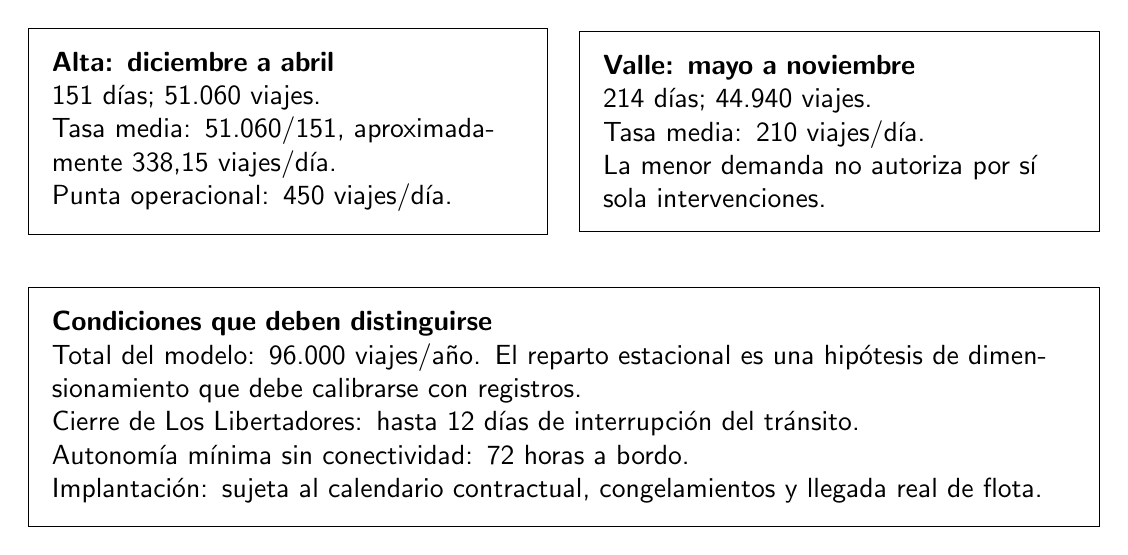
\begin{tikzpicture}[every node/.style={draw,align=left,text width=60mm,inner sep=3mm,font=\sffamily\fontsize{9.5bp}{12bp}\selectfont}]
\node at (0,0) {\textbf{Alta: diciembre a abril}\\151 días; 51.060 viajes.\\Tasa media: 51.060/151, aproximadamente 338,15 viajes/día.\\Punta operacional: 450 viajes/día.};
\node at (7,0) {\textbf{Valle: mayo a noviembre}\\214 días; 44.940 viajes.\\Tasa media: 210 viajes/día.\\La menor demanda no autoriza por sí sola intervenciones.};
\node[text width=130mm] at (3.5,-3.5) {\textbf{Condiciones que deben distinguirse}\\Total del modelo: 96.000 viajes/año. El reparto estacional es una hipótesis de dimensionamiento que debe calibrarse con registros.\\Cierre de Los Libertadores: hasta 12 días de interrupción del tránsito.\\Autonomía mínima sin conectividad: 72 horas a bordo.\\Implantación: sujeta al calendario contractual, congelamientos y llegada real de flota.};
\end{tikzpicture}
\par\smallskip Fuente: Caso 10 y modelo de demanda de audIT.
\end{figuraNativa}

\begin{figuraNativa}[htbp]{Cadena causal integrada de patologías sistémicas y pérdida de valor}{2-cadena-causal}
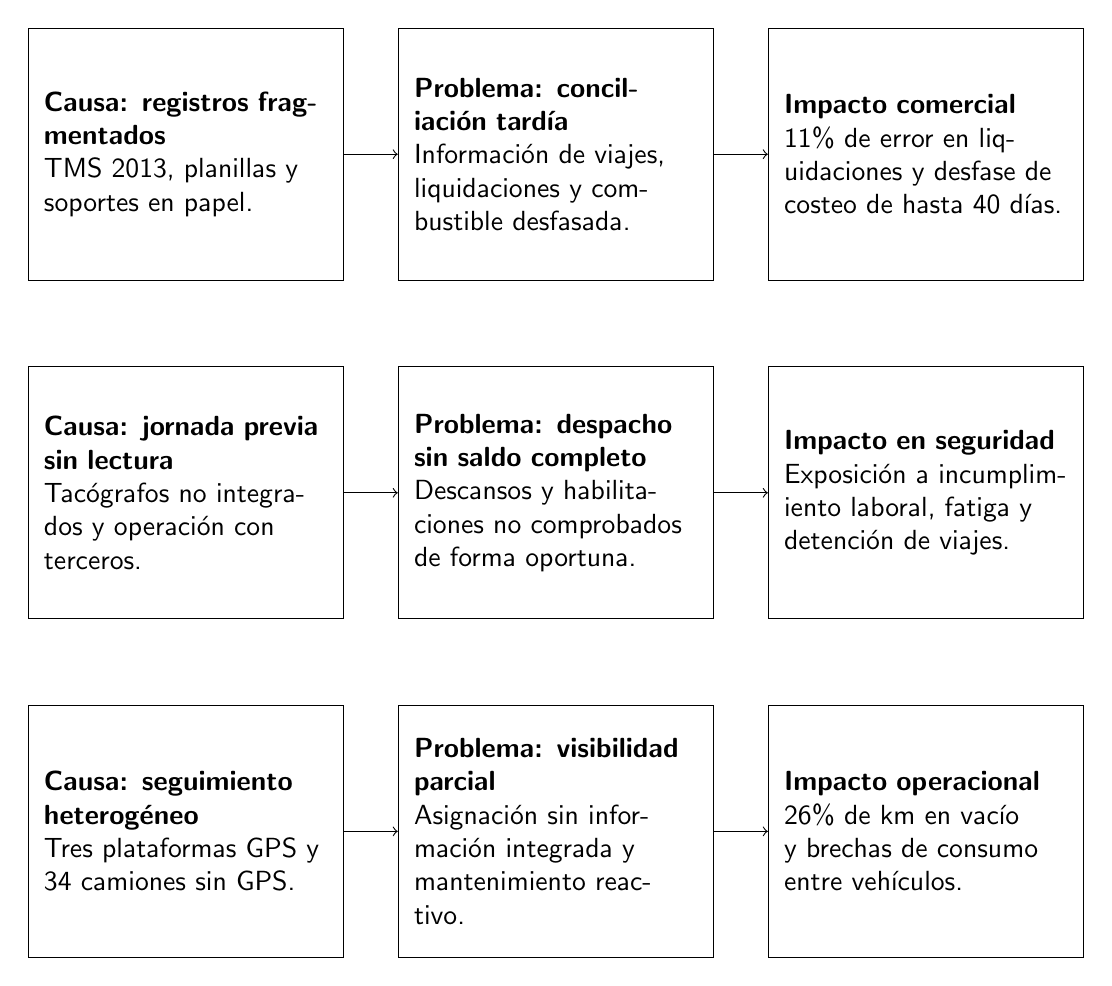
\begin{tikzpicture}[every node/.style={draw,align=left,text width=36mm,inner sep=2mm,minimum height=32mm,font=\sffamily\fontsize{9.5bp}{12bp}\selectfont}]
\node (a) at (0,0) {\textbf{Causa: registros fragmentados}\\TMS 2013, planillas y soportes en papel.};
\node (b) at (4.7,0) {\textbf{Problema: conciliación tardía}\\Información de viajes, liquidaciones y combustible desfasada.};
\node (c) at (9.4,0) {\textbf{Impacto comercial}\\11\% de error en liquidaciones y desfase de costeo de hasta 40 días.};
\node (d) at (0,-4.3) {\textbf{Causa: jornada previa sin lectura}\\Tacógrafos no integrados y operación con terceros.};
\node (e) at (4.7,-4.3) {\textbf{Problema: despacho sin saldo completo}\\Descansos y habilitaciones no comprobados de forma oportuna.};
\node (f) at (9.4,-4.3) {\textbf{Impacto en seguridad}\\Exposición a incumplimiento laboral, fatiga y detención de viajes.};
\node (g) at (0,-8.6) {\textbf{Causa: seguimiento heterogéneo}\\Tres plataformas GPS y 34 camiones sin GPS.};
\node (h) at (4.7,-8.6) {\textbf{Problema: visibilidad parcial}\\Asignación sin información integrada y mantenimiento reactivo.};
\node (i) at (9.4,-8.6) {\textbf{Impacto operacional}\\26\% de km en vacío y brechas de consumo entre vehículos.};
\draw[->] (a.east)--(b.west);\draw[->] (b.east)--(c.west);
\draw[->] (d.east)--(e.west);\draw[->] (e.east)--(f.west);
\draw[->] (g.east)--(h.west);\draw[->] (h.east)--(i.west);
\end{tikzpicture}
\par\smallskip Fuente: Elaboración propia a partir del diagnóstico del Caso 10.
\end{figuraNativa}

\begin{figuraNativa}[htbp]{Poder efectivo e interés operativo de los 13 actores de Curimón}{2-matriz-actores}
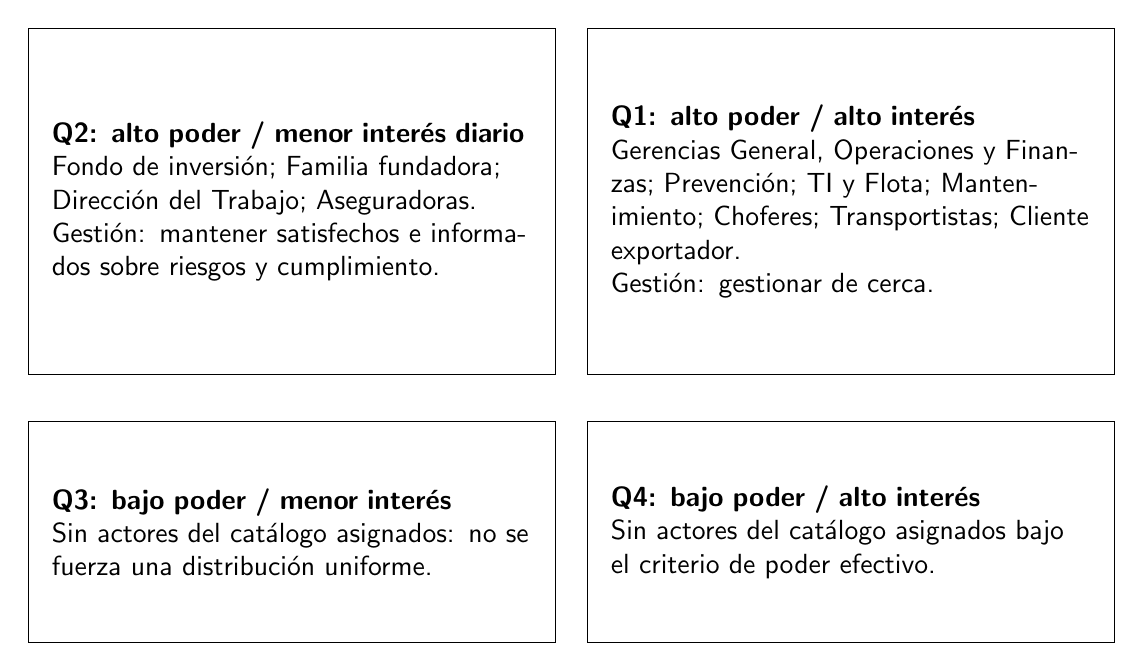
\begin{tikzpicture}[every node/.style={font=\sffamily\fontsize{9.5bp}{12bp}\selectfont,align=left}]
\node[draw,text width=61mm,inner sep=3mm,minimum height=44mm] at (0,0) {\textbf{Q2: alto poder / menor interés diario}\\Fondo de inversión; Familia fundadora; Dirección del Trabajo; Aseguradoras.\\Gestión: mantener satisfechos e informados sobre riesgos y cumplimiento.};
\node[draw,text width=61mm,inner sep=3mm,minimum height=44mm] at (7.1,0) {\textbf{Q1: alto poder / alto interés}\\Gerencias General, Operaciones y Finanzas; Prevención; TI y Flota; Mantenimiento; Choferes; Transportistas; Cliente exportador.\\Gestión: gestionar de cerca.};
\node[draw,text width=61mm,inner sep=3mm,minimum height=28mm] at (0,-4.2) {\textbf{Q3: bajo poder / menor interés}\\Sin actores del catálogo asignados: no se fuerza una distribución uniforme.};
\node[draw,text width=61mm,inner sep=3mm,minimum height=28mm] at (7.1,-4.2) {\textbf{Q4: bajo poder / alto interés}\\Sin actores del catálogo asignados bajo el criterio de poder efectivo.};
\end{tikzpicture}
\par\smallskip Fuente: Elaboración propia a partir de las entrevistas y poblaciones del Caso 10.
\end{figuraNativa}